\section{Aplicación Web (Servidor)}

El sistema del Administrador tiene como finalidad el poder gestionar los usuarios,servicios y de listas de equipaje.
Esto permite tener el control sobre los contenidos que el Usuario puede ver desde su aplicación móvil. También, nos da la posibilidad
de extender la información referente a los servicios dentro del AICM-T1 y, en general, mantenerla actualizada sin importar los cambios
que se vayan dando en el AICM-T1.

Por último, es importante mencionar que este módulo incluso nos permite agregar y gestionar sugerencias de listas de equipaje útiles 
para el viajero. Además de mantener un control sobre el número de usuarios de la aplicación.

\subsection{Generalidades}
El sistema de Administración utiliza las siguientes tecnologías para llevar a cabo sus funciones:
\begin{itemize}
 \item Lenguaje de programación PHP, combinando HTML, CSS3 y Javascript.
 \item JSON para el envío de información a la aplicación móvil TASMC.
 \item Hosting gratuito de Hostinger para alojar la aplicación web TASMC y el servicio web TASMC.
\end{itemize}

\subsection{Funcionalidades}

\subsubsection{Iniciar Sesión}
El administrador deberá ingresar su correo y contraseña que le fueron asignados para la gestión de los recursos de la aplicación. A partir 
de ello se mostrará una página principal la cual contiene un menú para ingresar a los distintos módulos.

\begin{figure}[h!]
	\centering
		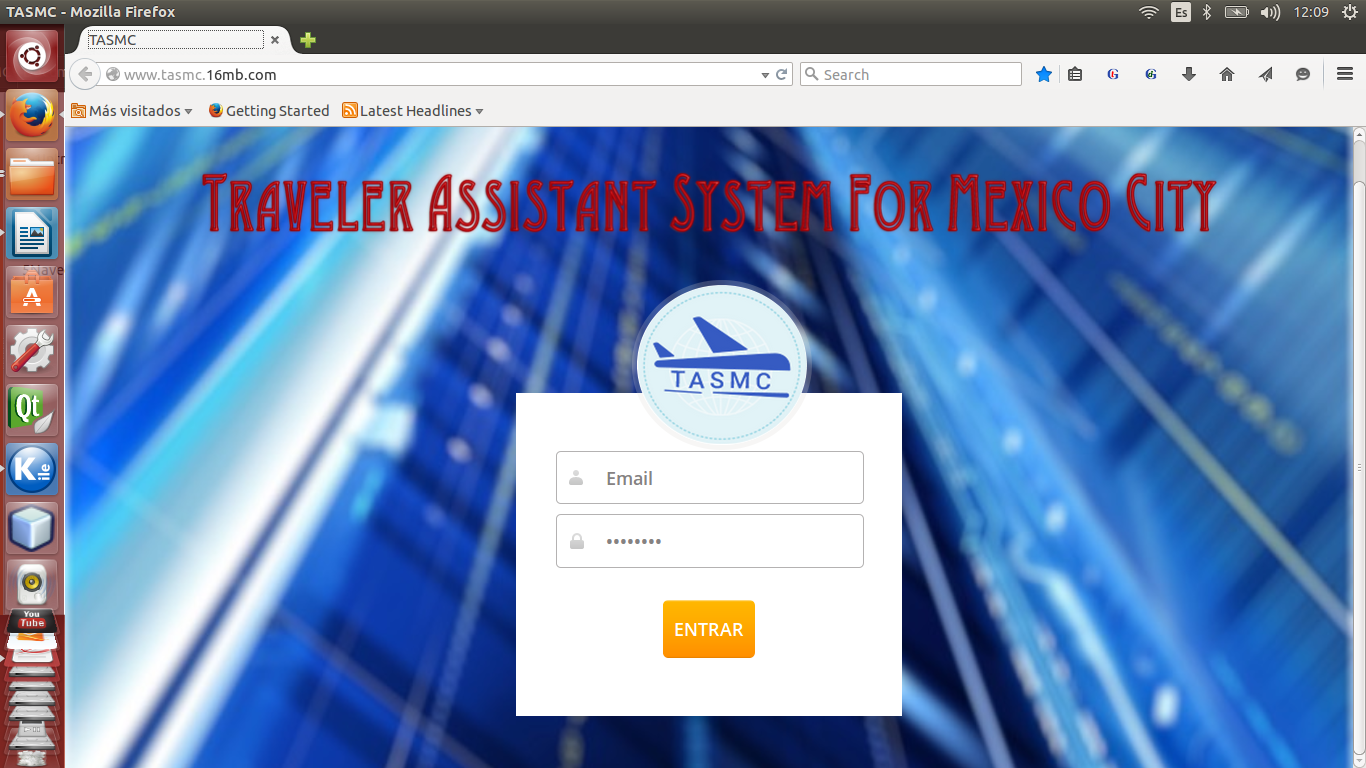
\includegraphics[width=0.8\textwidth]{Figuras/principalTASMC.png}
		\rule{35em}{0.5pt}
	\caption[Iniciar sesión aplicación web]{Iniciar sesión aplicación web}
	\label{fig:vistaInicio}
\end{figure}
\clearpage

\begin{figure}[h!]
	\centering
		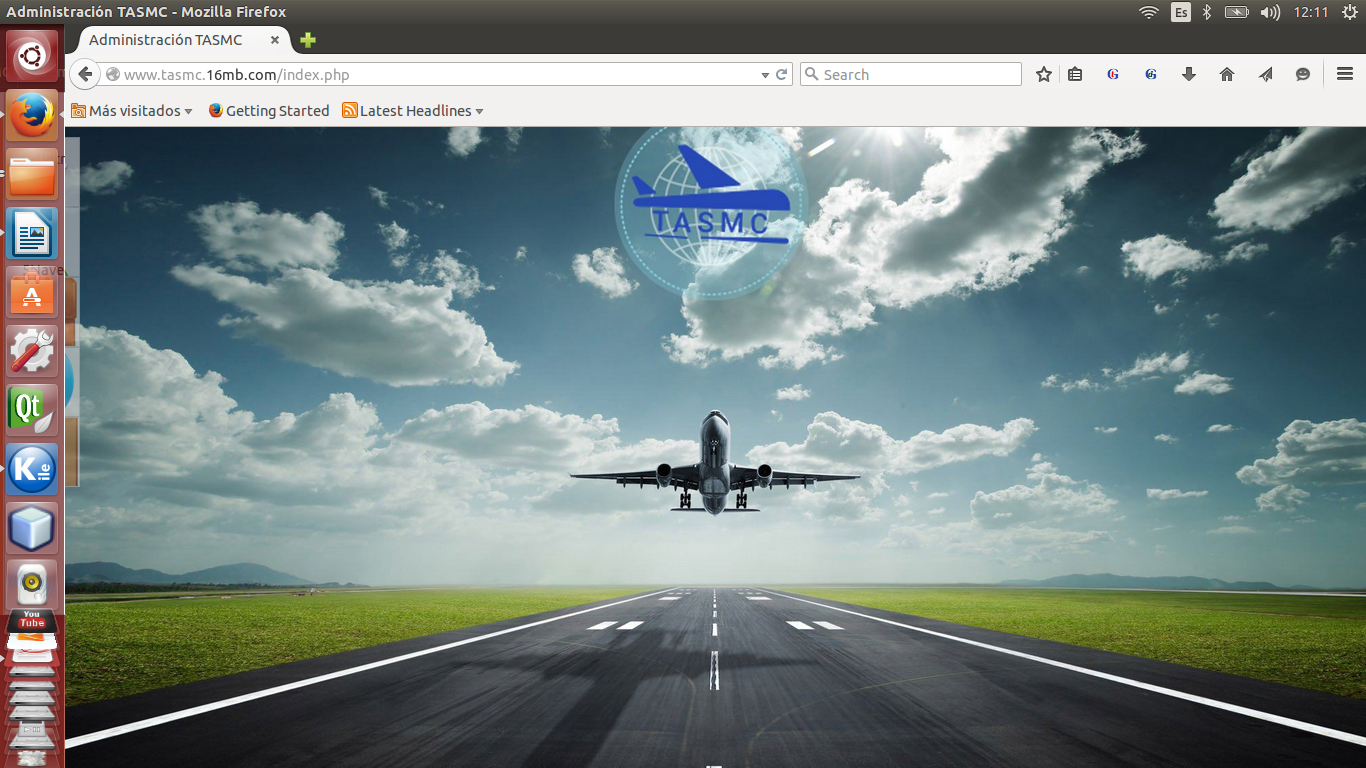
\includegraphics[width=0.8\textwidth]{Figuras/index.png}
		\rule{35em}{0.5pt}
	\caption[Página principal TASMC]{Página principal TASMC}
	\label{fig:indexWeb}
\end{figure}
\begin{figure}[h!]
	\centering
		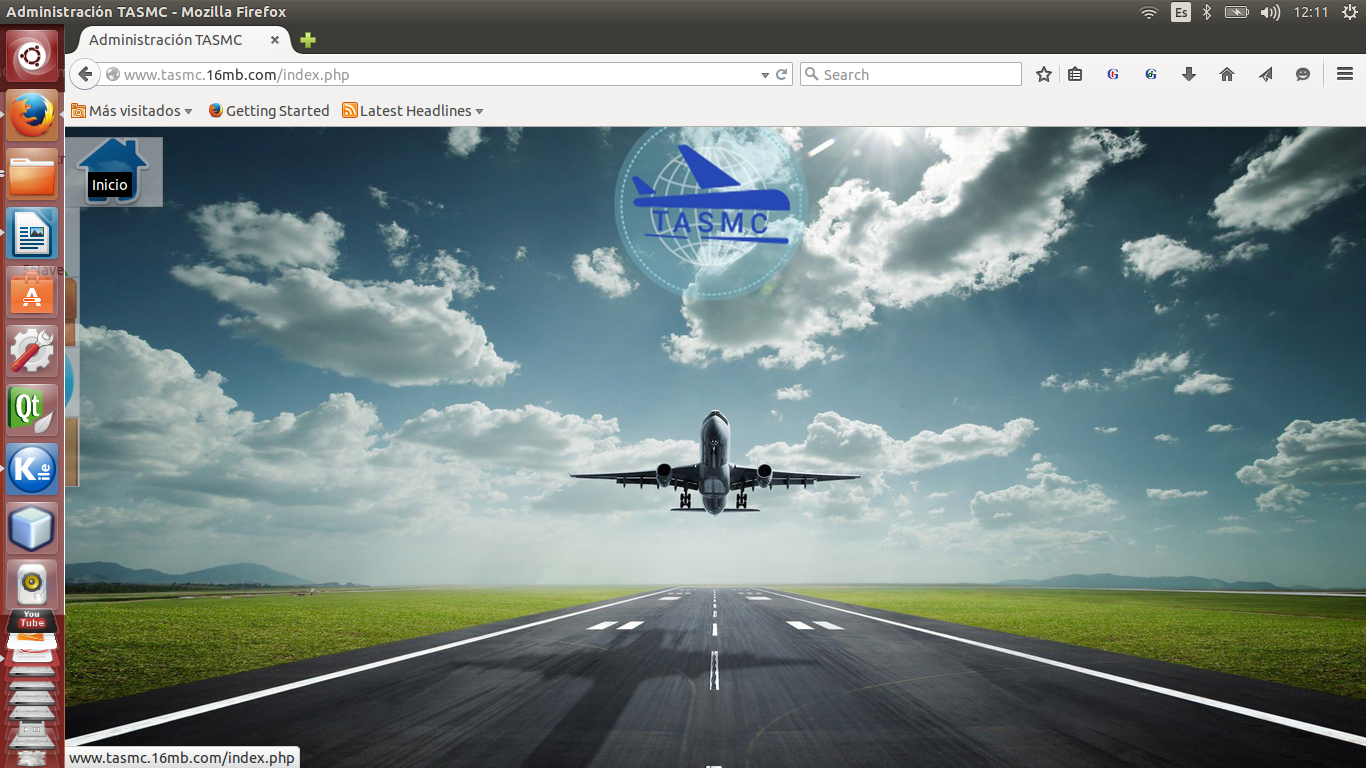
\includegraphics[width=0.8\textwidth]{Figuras/indexhome.png}
		\rule{35em}{0.5pt}
	\caption[Menú Inicio]{Menú Inicio}
	\label{fig:menuInicio}
\end{figure}
\clearpage

\subsubsection{Gestionar Usuario}
Está sección será únicamente de verficación, es decir, para tener un seguimiento y control de los usuarios activos de la aplicación móvil 
mediante un campo de última visita que muestra la hora y fecha en la cual el usuario uso la aplicación por última vez.
\begin{figure}[h!]
	\centering
		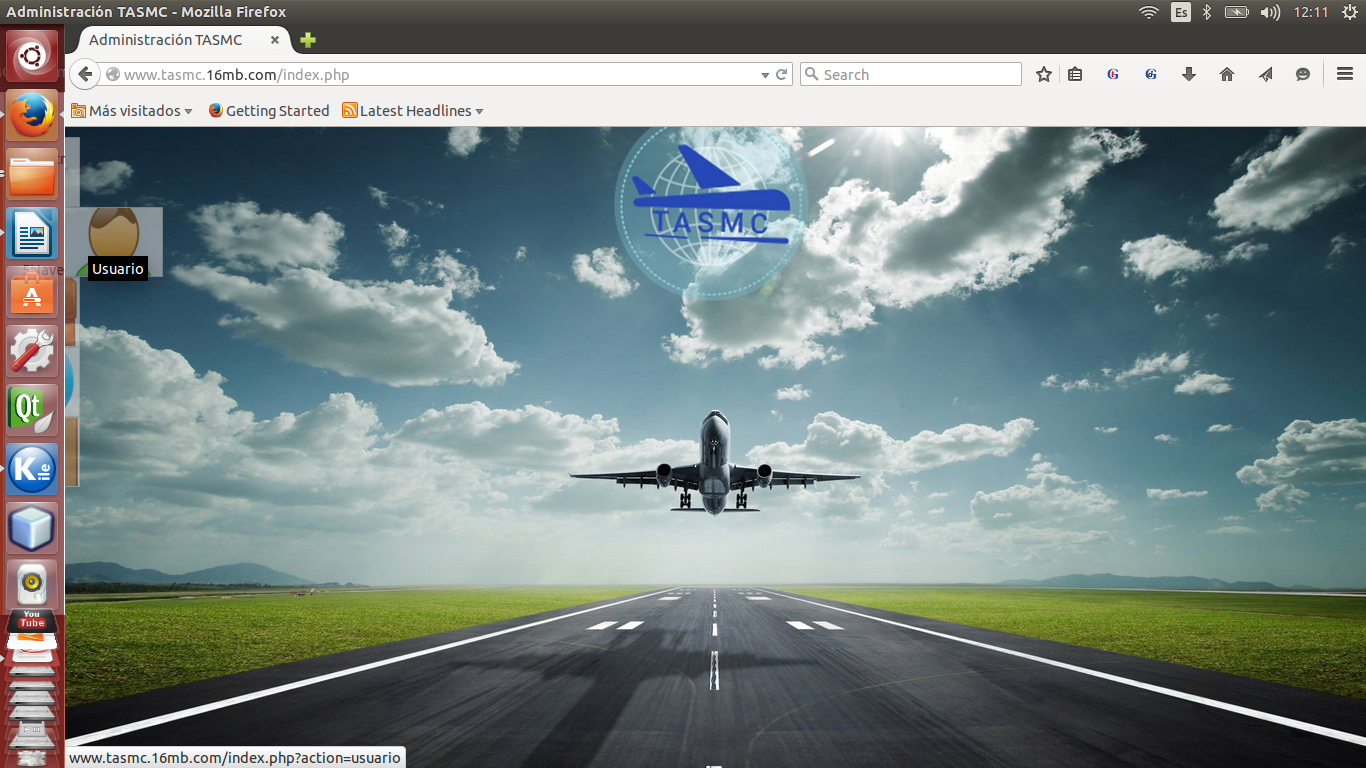
\includegraphics[width=0.8\textwidth]{Figuras/indexUsuario.png}
		\rule{35em}{0.5pt}
	\caption[Menú Usuario]{Menú Usuario}
	\label{fig:menuUsuario}
\end{figure}
\begin{figure}[h!]
	\centering
		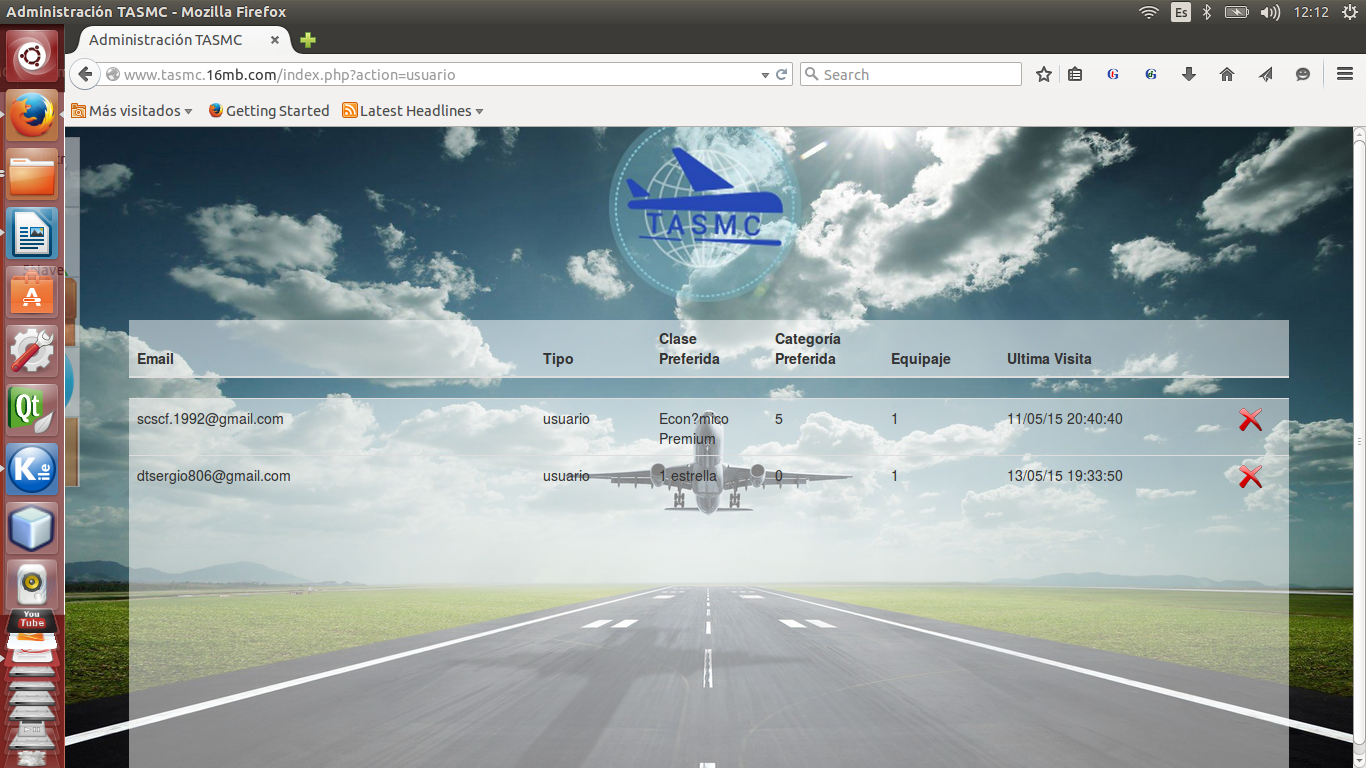
\includegraphics[width=0.8\textwidth]{Figuras/usuarios.png}
		\rule{35em}{0.5pt}
	\caption[Módulo Gestión de Usuarios]{Módulo Gestión de Usuarios}
	\label{fig:moduloUsuarios}
\end{figure}
\clearpage

\subsubsection{Gestionar Equipaje}
En este módulo el admnistrador puede crear nuevas sugerencias de listas de equipaje, cada una con distintos tipos de objetos separados 
por categoría, además de poder crear nuevos objetos asociados a una categoría específica. Las listas de sugerencia de equipaje estarán 
reflejadas dentro de la aplicación móvil pero las listas creadas propias del usuario no se mostrarán en la aplicación web.
\begin{figure}[h!]
	\centering
		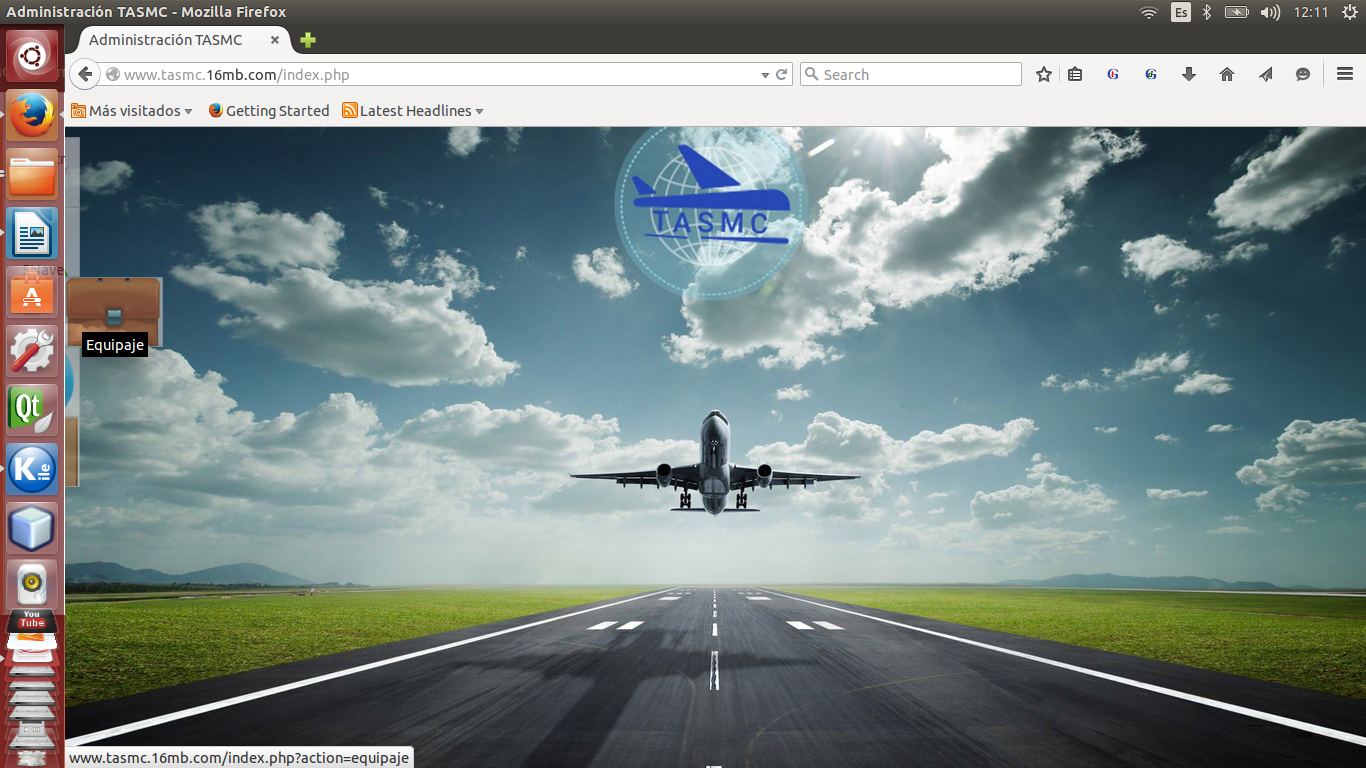
\includegraphics[width=0.8\textwidth]{Figuras/indexEquipaje.png}
		\rule{35em}{0.5pt}
	\caption[Menú Equipaje]{Menú Equipaje}
	\label{fig:menuEquipaje}
\end{figure}
\begin{figure}[h!]
	\centering
		
\includegraphics[width=0.8\textwidth]{Figuras/equipajes.png}
		\rule{35em}{0.5pt}
	\caption[Módulo Gestión de Equipaje]{Módulo Gestión de Equipaje}
	\label{fig:moduloEquipaje}
\end{figure}

\begin{figure}[h!]
	\centering
		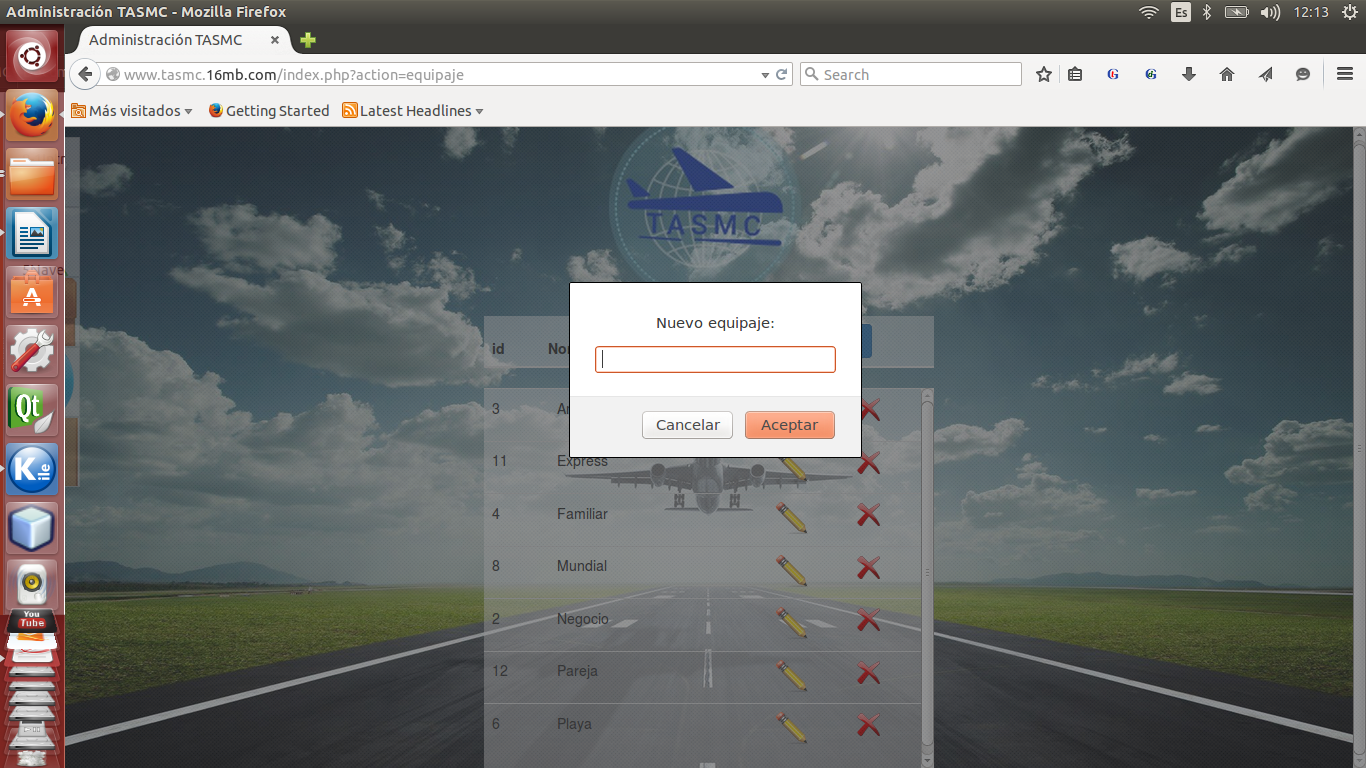
\includegraphics[width=0.8\textwidth]{Figuras/nuevoequipajewb.png}
		\rule{35em}{0.5pt}
	\caption[Función de creación de nuevo equipaje]{Función de creación de nuevo equipaje}
	\label{fig:funcionNuevoEquipaje}
\end{figure}

\begin{figure}[h!]
	\centering
		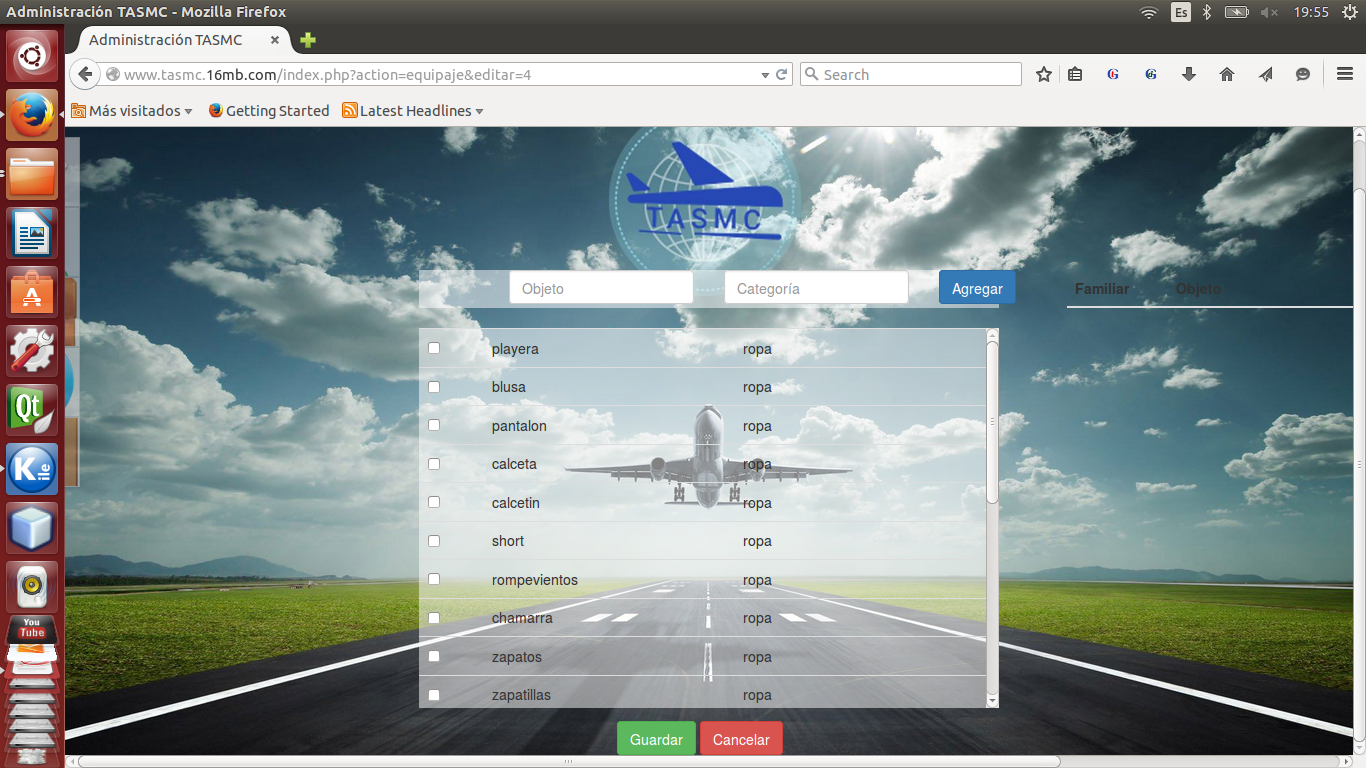
\includegraphics[width=0.8\textwidth]{Figuras/objetosEquipaje.png}
		\rule{35em}{0.5pt}
	\caption[Módulo de Gestión de objetos de equipaje]{Módulo de Gestión de objetos de equipaje}
	\label{fig:moduloObjetos}
\end{figure}
\clearpage

\subsubsection{Gestionar Servicio}
En esté módulo se añade la información correspondiente a los distintos servicios con los cuales cuenta el AICM-T1, como es: 
\begin{itemize}
 \item Nombre
 \item Rango de Precios
 \item Local
 \item Categoría
 \item Teléfono
 \item Horario
\end{itemize}

\begin{figure}[h!]
	\centering
		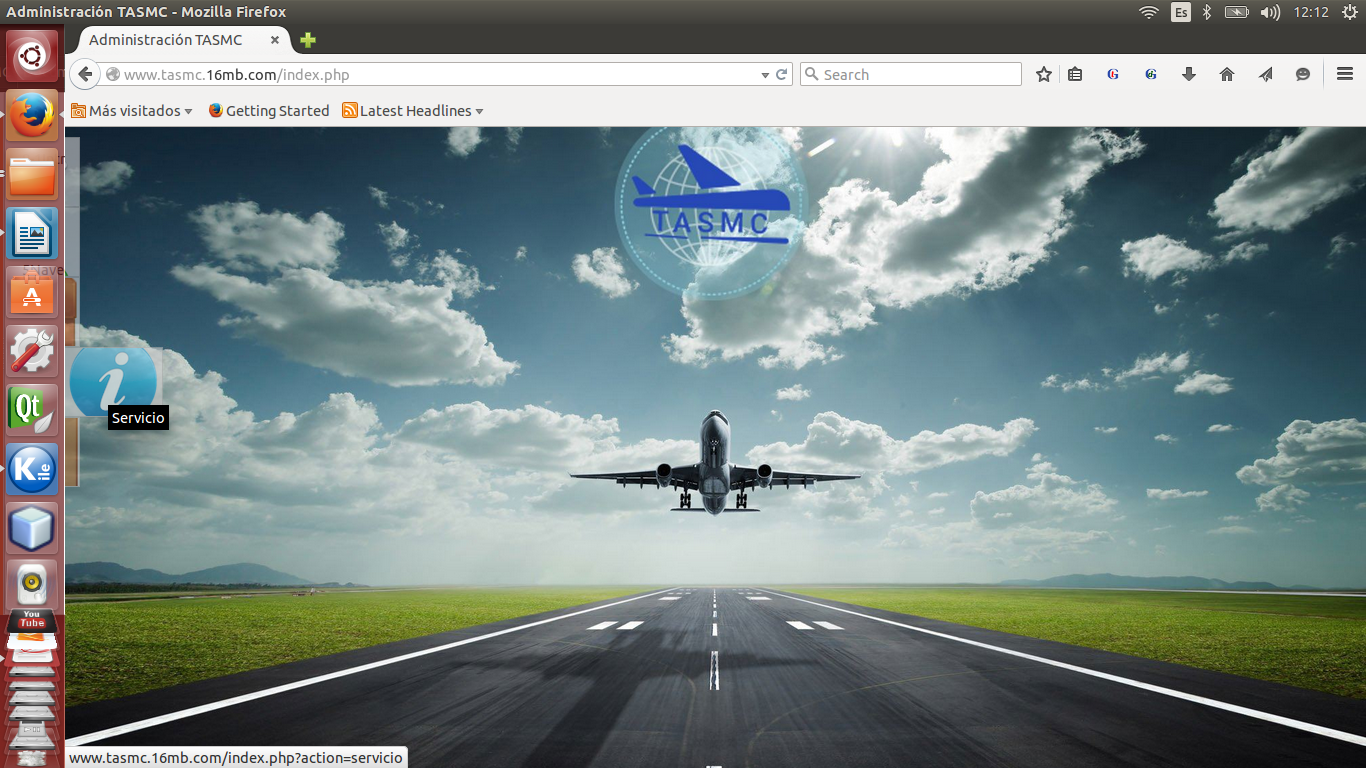
\includegraphics[width=0.8\textwidth]{Figuras/indexServicio.png}
		\rule{35em}{0.5pt}
	\caption[Menú Servicio]{Menú Servicio}
	\label{fig:menuServicio}
\end{figure}

\begin{figure}[h!]
	\centering
		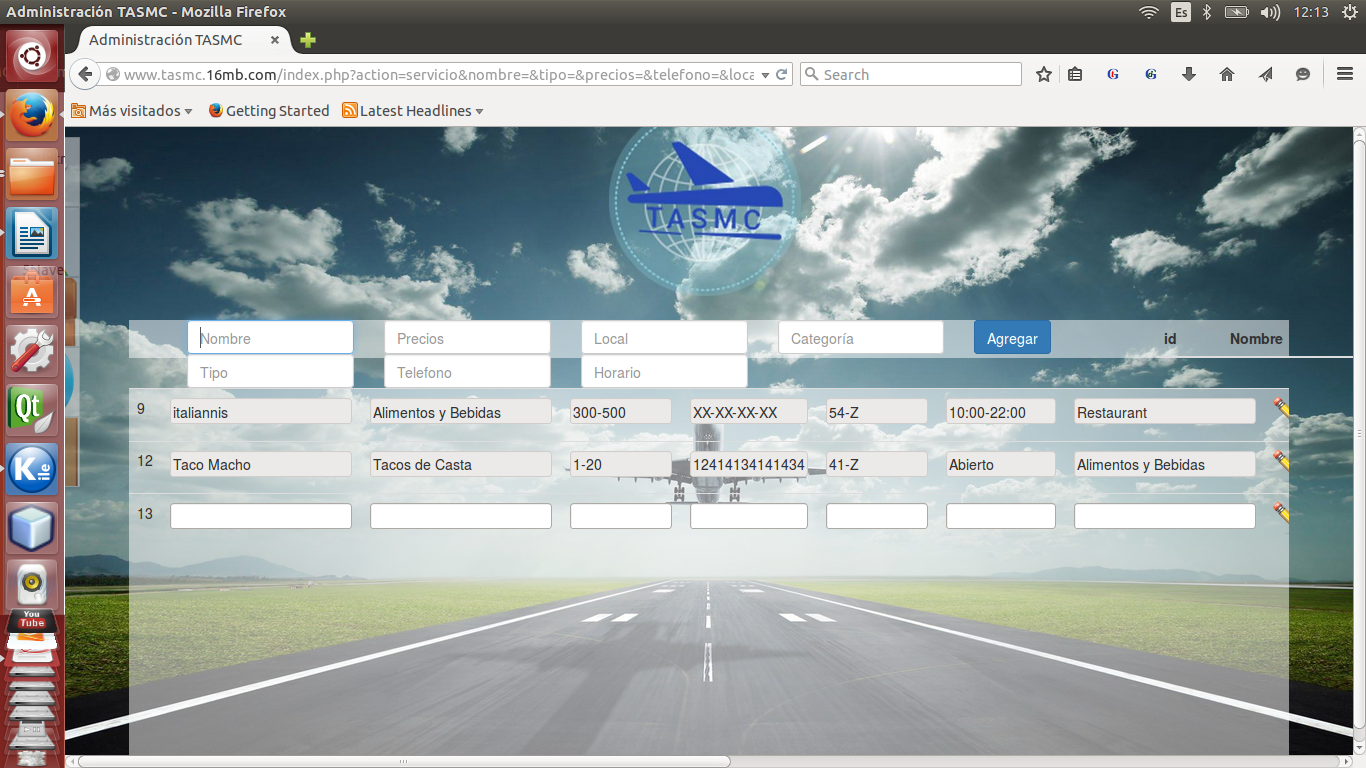
\includegraphics[width=0.8\textwidth]{Figuras/servicioswb.png}
		\rule{35em}{0.5pt}
	\caption[Módulo Gestión de Servicios]{Módulo Gestión de Servicios}
	\label{fig:moduloUsuarios}
\end{figure}

\subsubsection{Cerrar Sesión}
El administrador termina su actividad de gestión dentro de la aplicación y cierra sesión.
\begin{figure}[h!]
	\centering
		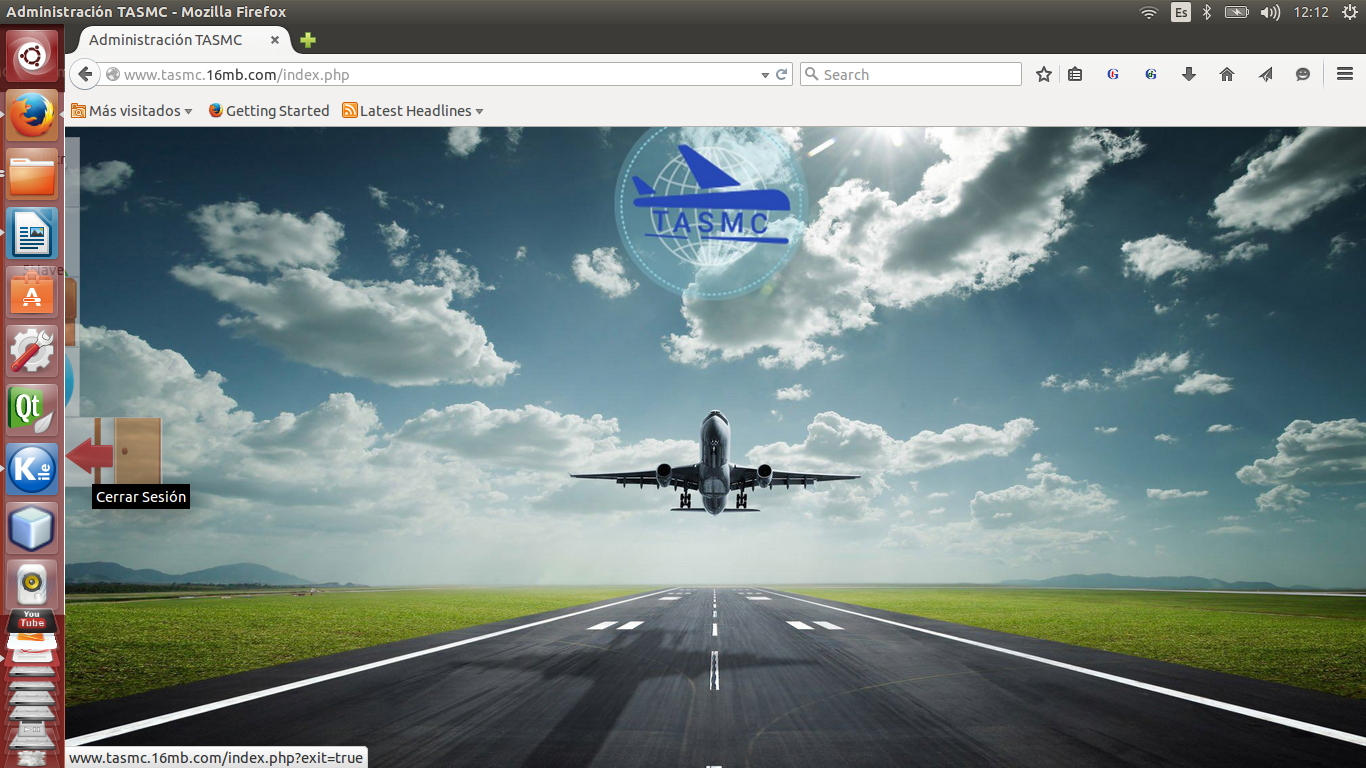
\includegraphics[width=0.8\textwidth]{Figuras/indexCerrarSesion.png}
		\rule{35em}{0.5pt}
	\caption[Menú Cerrar Sesión]{Menú Cerrar Sesión}
	\label{fig:menuCerrar}
\end{figure}
\clearpage

\section{Servicio Web TRASO}

Se creó un servicio web para añadir las funcionalidades de búsqueda de hoteles, búsqueda de vuelos y consulta de vuelos. La implementación de TRASO es consecuencia de la nula respuesta por parte de Amadeus Web Services. 

La información que TRASO brinda a la aplicación móvil no es real, como se tenía planeado al inicio del trabajo terminal, sin embargo cumple con la funcionalidad esperada. 

El modelo relacional de la base de datos creada para este servicio web se puede visualizar en la Figura \ref{fig:relacionalTRASO}.

\subsection{Generalidades}
El servicio web TRASO utiliza las siguientes tecnologías para llevar a cabo sus funciones:
\begin{itemize}
 \item Lenguaje de programación PHP.
 \item JSON para el envío de información a la aplicación móvil TASMC.
 \item Hosting gratuito de Hostinger para alojar el servicio web TRASO.
\end{itemize}
\clearpage